\section{Angular dependency of the Rutherford cross section}
The Rutherford differential cross section \parencite[p. 16]{noteBB} is given by
\begin{align}\label{eq:cross}
    {\left( \diff[d]{\sigma}{\Omega} \right)}_|Rutherford| =
    {\left(\frac{Z_1Z_2 e^2}{4E_{\infty}} \right)}^2
    \frac{1}{{{\sin}^4(\frac{\theta}{2})}},
\end{align}
where $Z$ is the proton number of each interacting particle, $E_{\infty}$ is
the asymptotic energy, and $\theta$ is the scattering angle. If the energy is
in units of $\si{\mega\electronvolt}$, this differential cross section will be in units
of $\si{\milli\barn\per\steradian}$.\\
This formula neglects the recoil energy of the target. 

As mentioned earlier, the target has two layers, and thus the incomming beam of
ions can scatter on both gold and carbon. 

However, as the Rutherford scattering is a coulomb interaction and $Z_|Au| >
Z_|C|$, the Rutherford differential cross section for gold is greater than for carbon at any given angle. Hence we would expect the gold layer to scatter more particles at higher angles compared to carbon. Due to the same inequality of the nuclei number gold will also have a lower recoil energy, and thus from conservation of energy the particles scattered on gold will have a higher energy - bin number - than carbon.
%Furthermore, from the calibration it is found that the channel numbers are directly proportional to the meassured energies of the scattered particles. Combined with the fact that gold has a higher nuclei number than carbon and thus a lower recoil energy, we will expect the particles scattered on gold will have a higher energy than those of carbon from conservation of energy.

%From the calibration it is found that the channel number is directly proportional to the energy of the scattered particles. Combined with the fact, that gold has a higher mass number, and thus a lower recoil energy, it is expected that the particles scattered on the gold layer will have a higher energy, due to conservation of energy.

%% %%

\subsection{Data analysis}
To test the angular dependency of the Rutherford differential cross section,
the Silicon detector was set at a variable angle. At each angle the total
number of incomming particles and scattered particles were measured.\\

A Faraday cup was used to meassure the amount of non-scattered particles. 
Since this number is far greater than the amount of scattered particles, the
number of incomming particles can be assumed to be the number of detected
particles within the Faraday cup.\\

The number of any detected events in both the Faraday cup and the Silicon
detector follows a Poisson distribution, and thus the statistical uncertainty
goes as the square root of the total number of detected events.\\

The counted events from the Faraday cup can be read off the collector. 
The collector was set to relate $10^{11}$ counts per coulomb, and as there are
$6,24150913\ \cdot10^{18}$ elementary
charges per coulomb, we can relate the count number to an amount of detected
protons, $N$. Due to the beampipe, a factor of one half is also
necesarry.\footnote{Hans Fynbo, course responsible, mentioned this factor,
    which surprisingly fit well into our calculations.}

The relation between the number of incoming, $N$, and scattered particles, $dN$, is
\begin{equation}\label{eq:dN}
    \mathrm{d}N = N n_|tar| \mathrm{d}x \mathrm{d}\Omega,
    \diff[d]{\sigma(\theta,\phi)}{\Omega}.
\end{equation}
\parencite[eq. 14.42, p. 582]{taylor} where $n_|tar|$ and $\mathrm{d}x$ is the
nuclei density of the target thickness of the target respectivly, and
$\mathrm{d}\Omega$ is the small solid angle through which the scattered
particles emerge.

As previously mentioned  the two layered target will result in a double
scattered profile, thus a fit is expected to follow a double gaussian
distribution. Asuming a linear combination of the two gaussians one can
describe the count distribution \cref{fig_doublegauss}.\\
\begin{figure}[h]
\centering
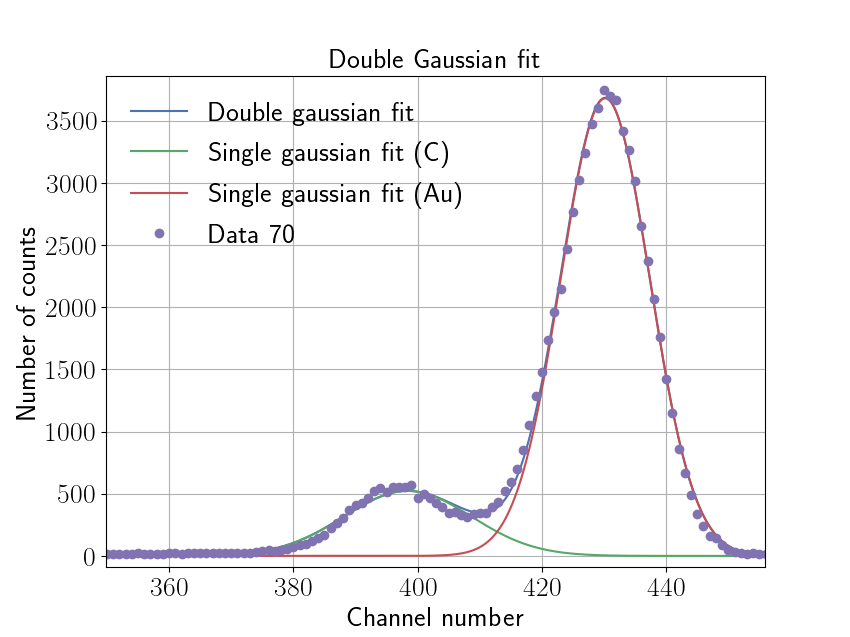
\includegraphics[width=0.99\columnwidth]{Data_70}
\caption{A double gaussian fit at a detector angle of $70$ degrees.}
\label{fig_doublegauss}
\end{figure}
Through a double gaussian fit we can distinguish between the scattered particles of gold and carbon, and determine their mean channel number corresponding to their energy.  \\
Fitting a double gaussian, one gather six parameters; amplitude, centroid and standard deviation
of both gaussians.  \\
%Notice in figure \ref{fig_angular_dependency} that the gaussian of greatest amplitude corresponds to gold, which
%is in agreement with the relative sizes of the two atoms. . Thus the recoil energy of gold is negligible compared to that of carbon.\\
Each gaussian term was used to determine the total count number by summing over
all channels, in order to obtain $\mathrm{d}N$ for particles scattered of gold
and carbon respectively.\\
%
From \cref{eq:dN} the differential cross section for each detector angle is
then calculated and compared to the expected differential cross section
\cref{eq:cross}.\\
\begin{figure}[h]
	\centering
		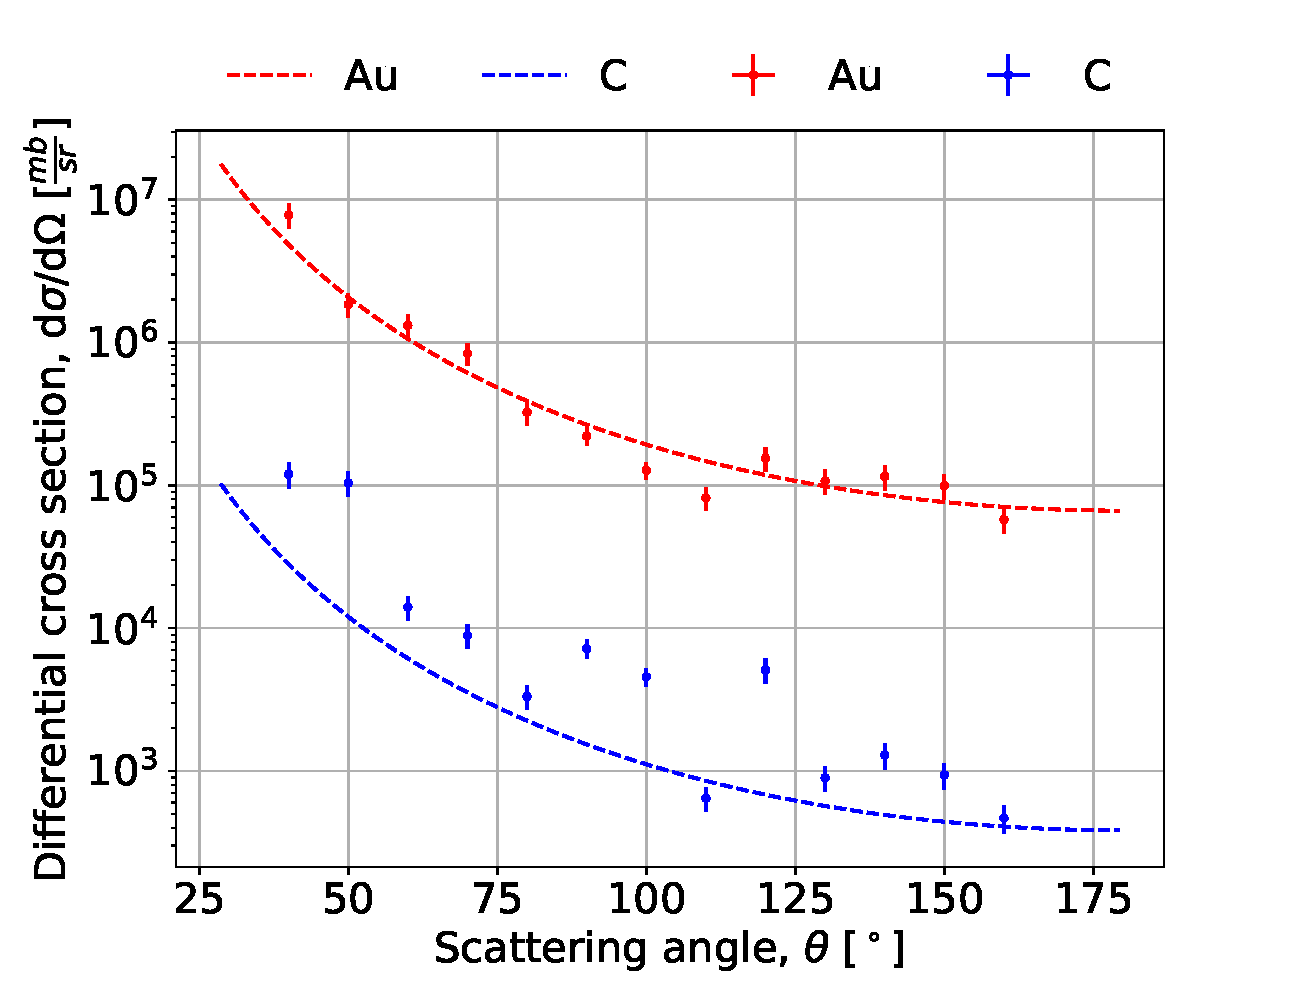
\includegraphics[width=0.45\textwidth]{Differential_cross_section.eps}
	\caption{The differential crossection  of carbon and gold as a function of the scattering angle. The dashed line represents the theoretical values.}
	\label{fig:Differential_cross_section}
\end{figure}
The data and the theoretical derived differential cross section have the same
characteristics though it seems as if all data for carbon is shifted to higher
values than what is expected by the theory.

The theoretical determined values are based on \cref{eq:cross}, which is under the assumption of a classical regime governt by the Sommerfeld criterion \parencite[p. 14]{noteBB}.
\begin{align}\label{eq:som}
\eta_|S|=0.16\cdot Z_1Z_2\sqrt{\frac{A_|proj|}{E_|lab|[\si{\mega\electronvolt}]}}\gg 1
\end{align}
For gold and carbon the values of the parameter is $\eta_|S|\sim 300$ and
$\eta_|S|\sim 6$ respectivly. It is interesting that the values for gold and carbon are in the order of $10^2$. Which could influence our theoretical assumptions for carbon. 

\section{Angular dependency of the proton energy}
From the double gaussian one obtains two centroids; one for each target layer.
These can be converted to the equivalent energies as described in the
calibration. Plotting the energy as a function of the detector angle
\cref{fig_energy}, it can be seen that the carbon layer radically changes
energies.
\begin{figure}[h!]
\centering
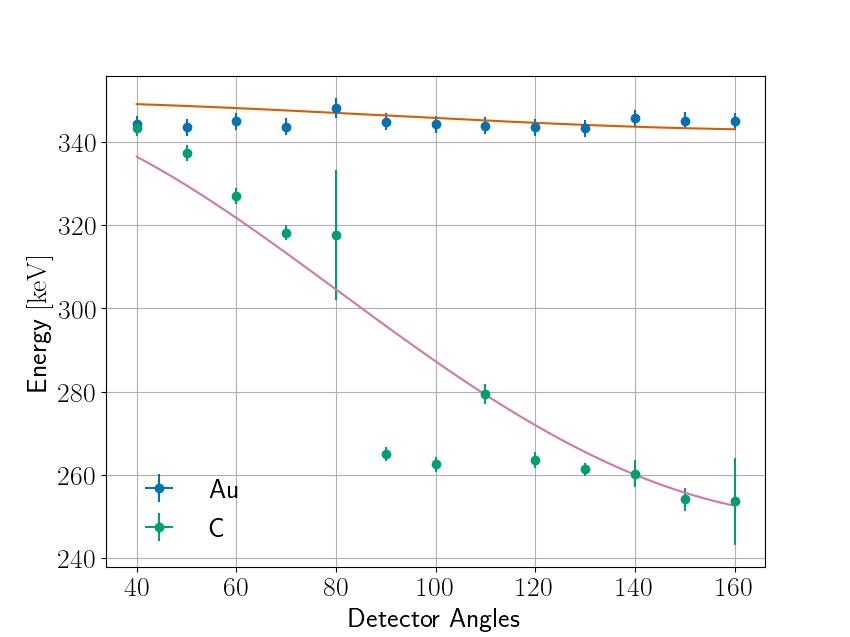
\includegraphics[width=0.99\columnwidth]{fig_energy}
\caption{Energies of Carbon and Gold scattered compared to theoretical
function.}
\label{fig_energy}
\end{figure}

On the otherhand gold is nearly constant. This is what is expected, as carbon
has a much higher recoil. Including the theoretical plot, as derived in
\cref{eq_5}, one can see that there exists some deviations from the expected
values. Especially at detector angles of $90$ and $100$ degrees.
A reason for this tendency, can be seen from \cref{fig_angular_dependency}. We
assume a linear combination of the gold and carbon distribution and thus fit a
double gaussian. Nonetheless, a small bump is seen between the carbon and gold
contributions. In a further analysis, one could fit a tripple gaussian and
identify the reason for this. The correction in bin number would shift it to
higher energy, which is just what would explain the lower energy than
expected.

Another interesting factor is how the two peaks change relative position as a
function of scattering, merging their gaussian distribution at low angles, \cref{fig_angular_dependency}. A complete overlap makes the seperation job more difficult, which explains the deviations at lower angles.


\begin{figure*}
\centering
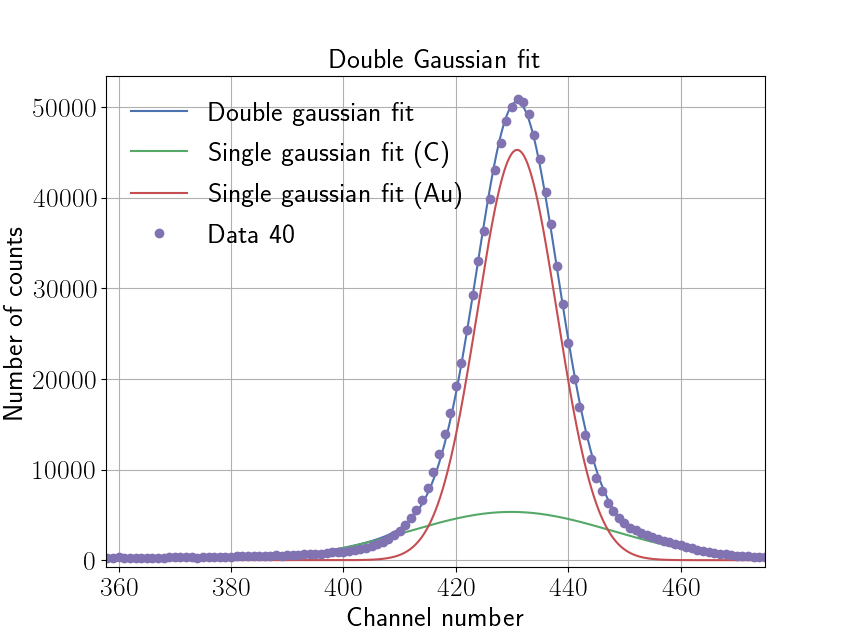
\includegraphics[width=0.99\columnwidth]{Data_40}
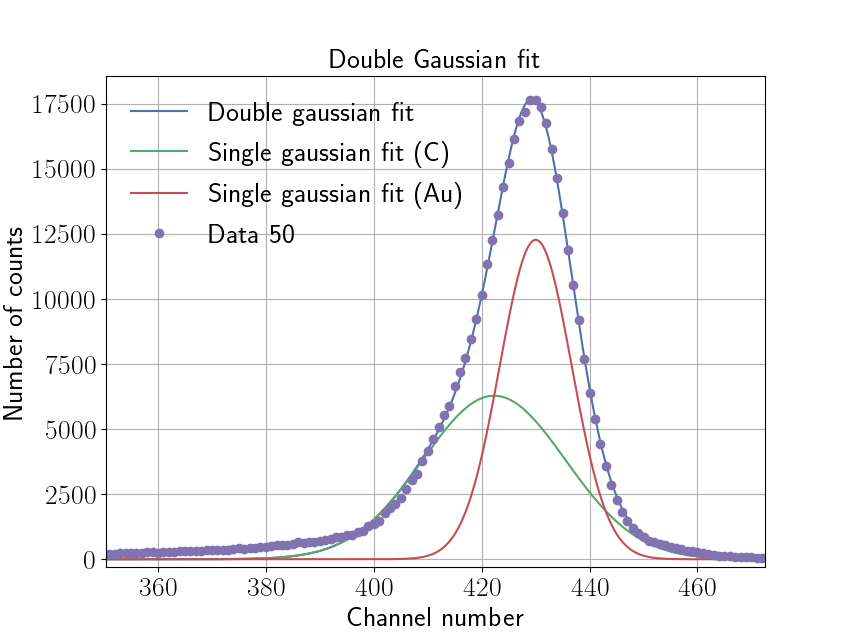
\includegraphics[width=0.99\columnwidth]{Data_50}
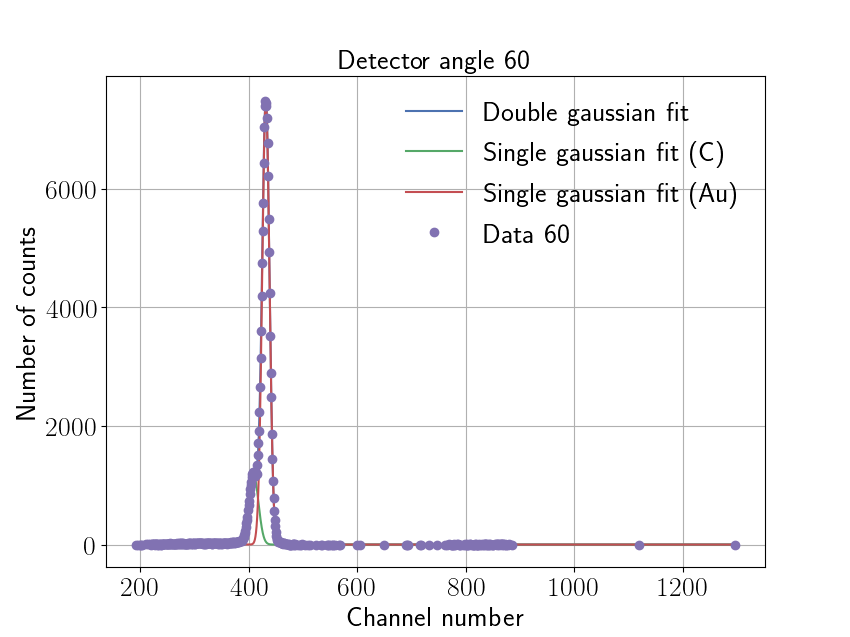
\includegraphics[width=0.99\columnwidth]{Data_60}
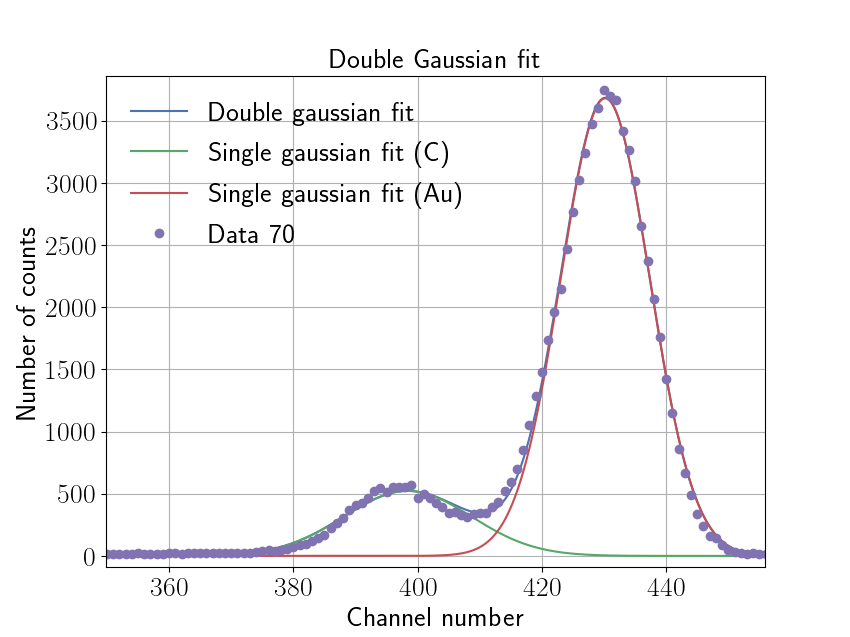
\includegraphics[width=0.99\columnwidth]{Data_70}
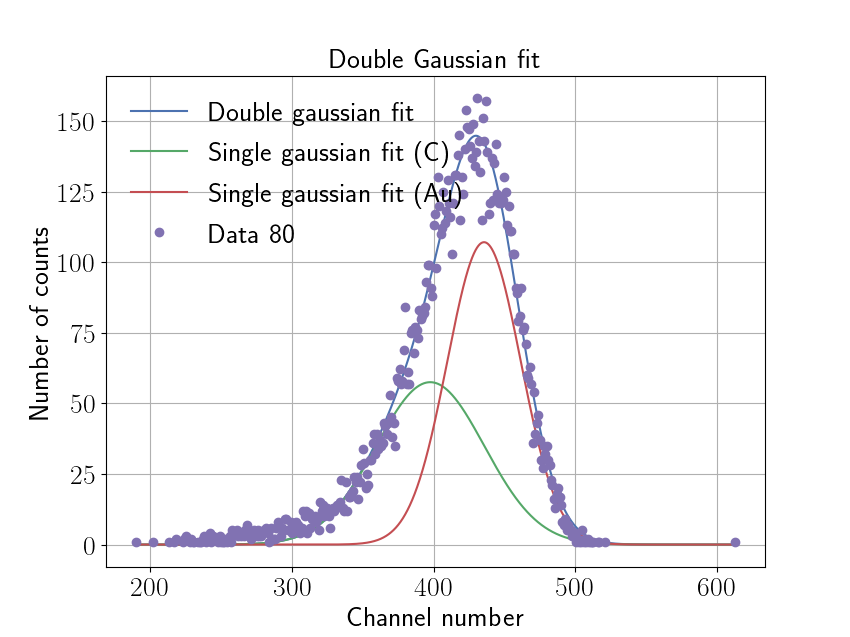
\includegraphics[width=0.99\columnwidth]{Data_80}
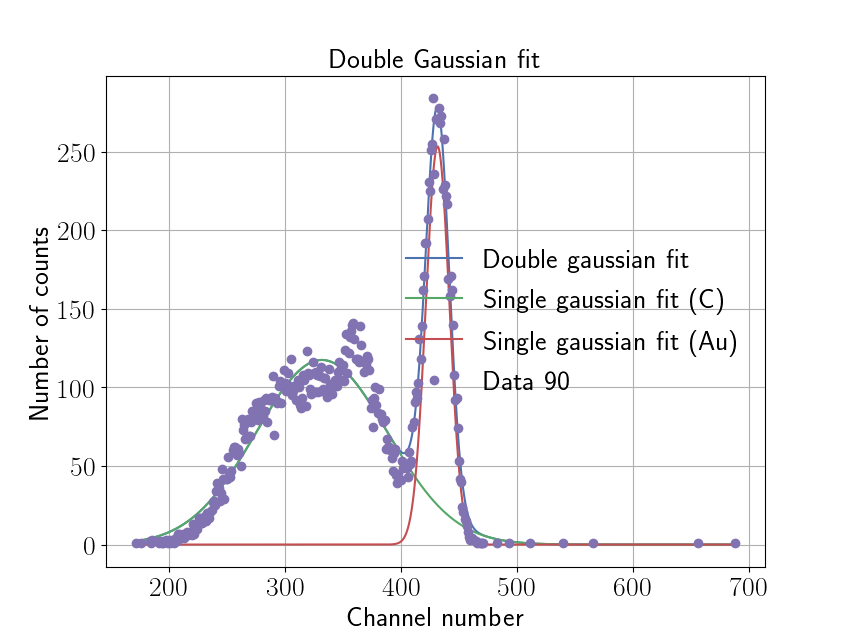
\includegraphics[width=0.99\columnwidth]{Data_90}
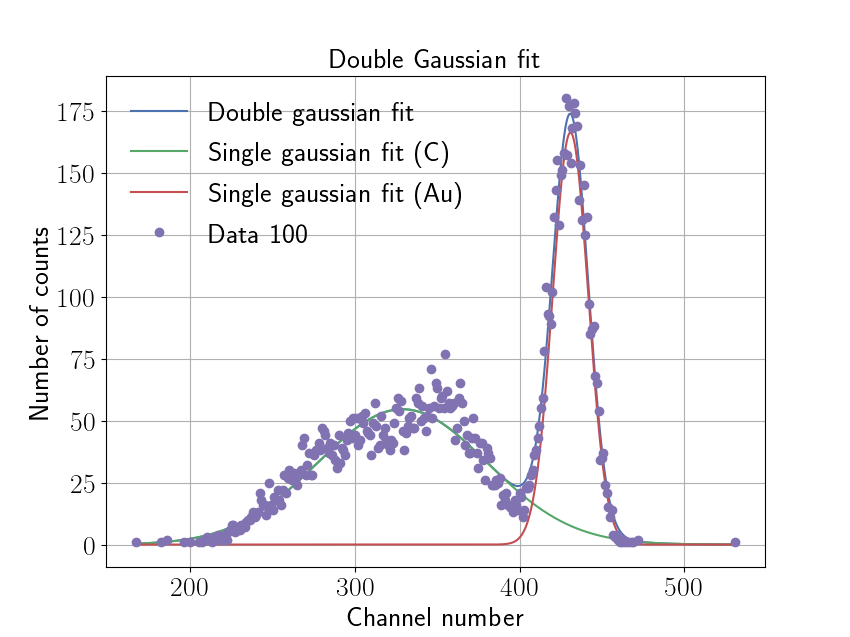
\includegraphics[width=0.99\columnwidth]{Data_100}
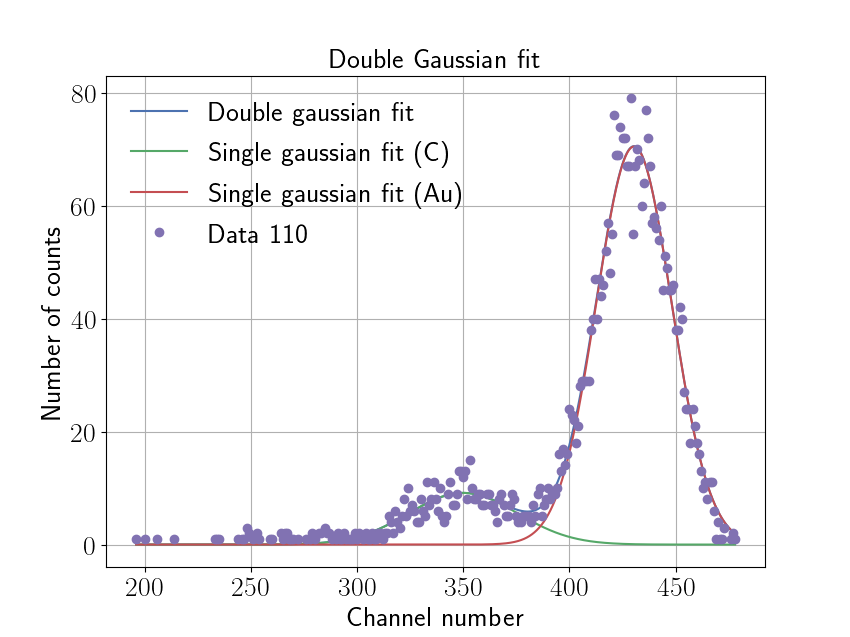
\includegraphics[width=0.99\columnwidth]{Data_110}
%\label{fig_angular_dependency}
\end{figure*}

\begin{figure*}
    \centering
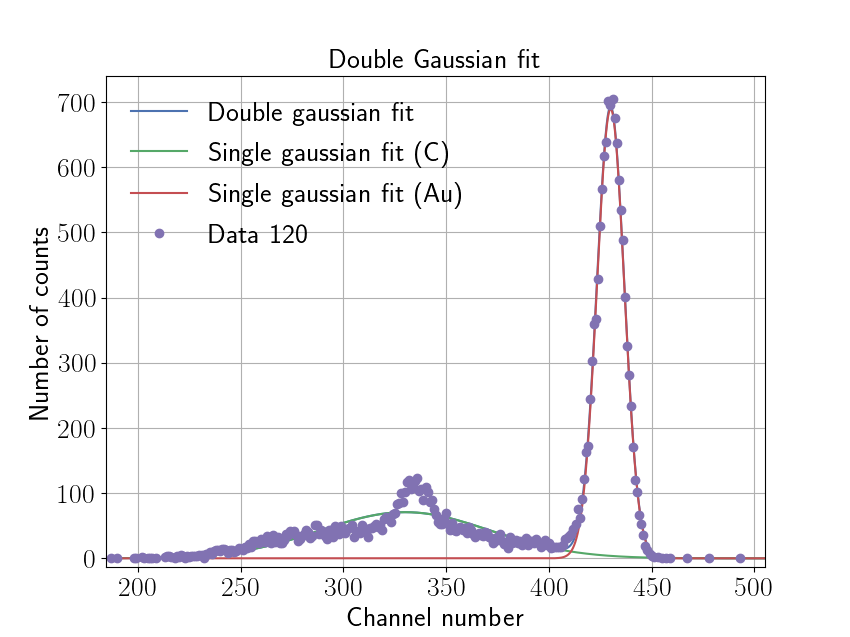
\includegraphics[width=0.99\columnwidth]{Data_120}
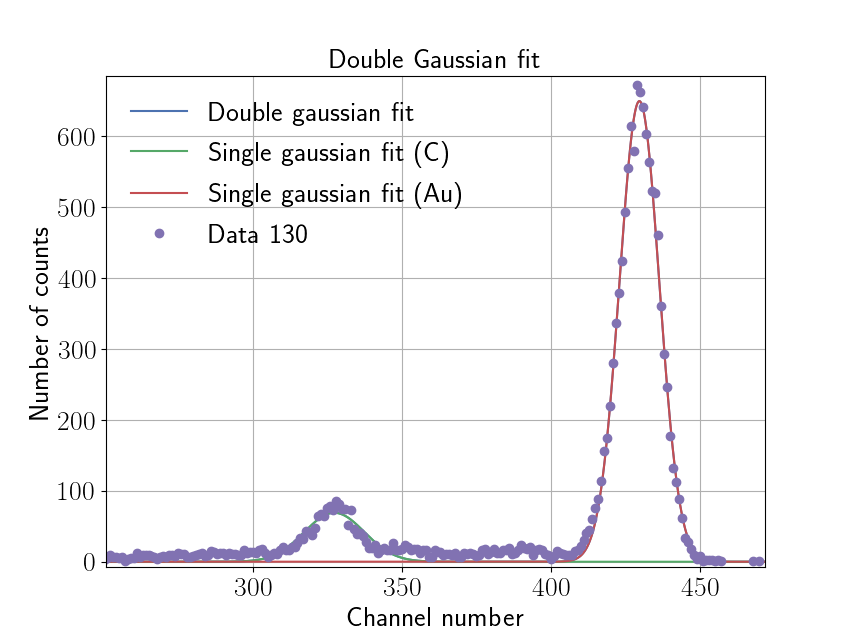
\includegraphics[width=0.99\columnwidth]{Data_130}
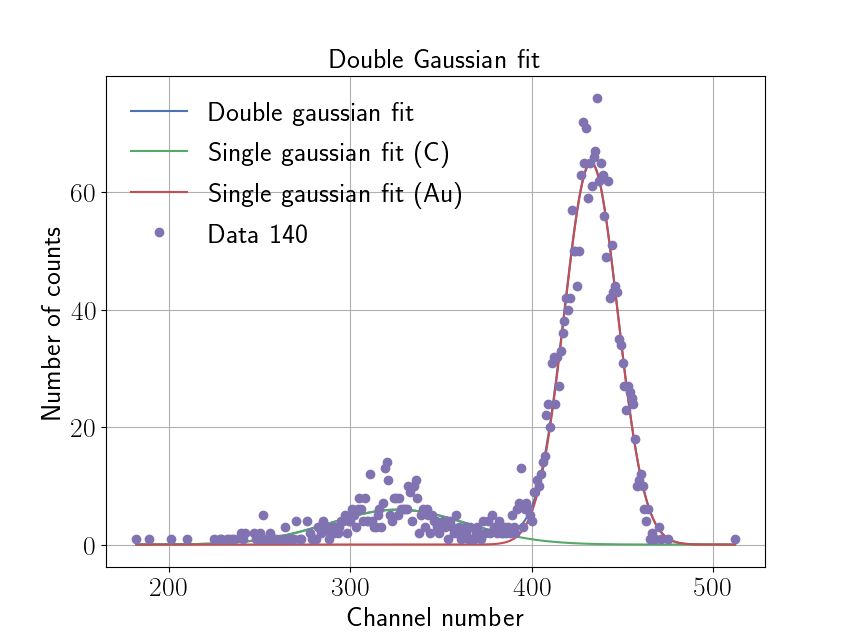
\includegraphics[width=0.99\columnwidth]{Data_140}
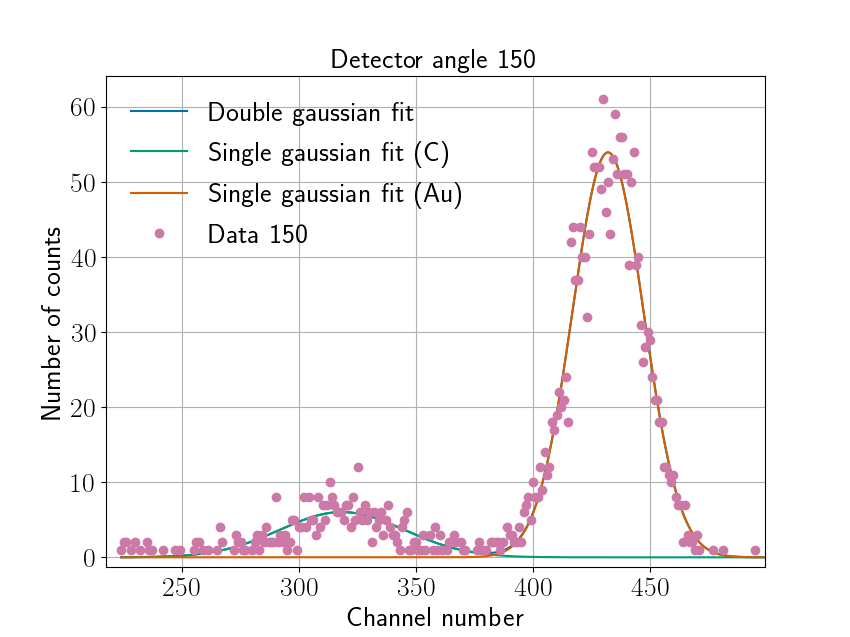
\includegraphics[width=0.99\columnwidth]{Data_150}
\caption{Angular dependency}
\label{fig_angular_dependency}
\end{figure*}
